\chapter{Absorber towards PG 0003+158} \label{ch:PG0003}

In this chapter, we describe a multi-component absorber system with a BLA candidate at $z\sim 0.347$ towards the line of sight of quasar PG 0003+158 ($z_{em}=0.4509$) which is a Sy1.2 AGN. We first fit the Voigt profiles to the absorption lines and then perform a detailed modelling of the ionization conditions in the absorber to know its ionisation state. We also analyse the galaxy neighbourhood of the absorber to understand the origins of the absorption system.   

\section{Component structure of the absorber system} \label{sec:component_structure}

We identified 3 components in the absorber system, i.e. three kinematically distinct absorption is seen. Table \ref{tab:components} lists the details of the components. We describe these components in subsequent sections.

\begin{table}
    \centering
    \begin{tabular}{ccc}
    \hline \hline 
    \head{Component}   &  \head{Ions} &  \head{$\mathbf{\Delta v \ (\text{km \ s}^{-1})}$} \\ 
    \hline \tabularnewline
         I    &                                     \ion{H}{i}                                       &   -163       \\
        II    &                             \ion{H}{i}, \ion{O}{vi}                                  &    0         \\ 
       III    &   \ion{H}{i}, \ion{O}{vi}, \ion{C}{ii}, \ion{C}{iii}, \ion{Si}{ii}, \ion{Si}{iii}    &    65        \\
    \tabularnewline \hline \hline \tabularnewline
    \end{tabular}
    \vspace*{-4mm}
    \caption{Component structure of the absorber system. Reference velocity at z = 0.347586}
    \label{tab:components}
\end{table}

\subsection{Component I : z $\sim$ 0.346776}

This component is the simplest of the 3 components as it is detected only in Ly $\alpha$ and Ly $\beta$ lines. Both the line are detected above 5$\sigma$ significance levels. This component lies at $\sim -180 \ \text{km s}^{-1}$ from the component II (from redshift of \ion{O}{vi} line : z = 0.347586). The other ions covered in COS coverage like \ion{N}{v}, \ion{C}{ii}, \ion{C}{iii}, \ion{Si}{ii}, \ion{Si}{iii}, \ion{Mg}{ii}, etc. are non-detections. Voigt profile fitting, as described in section \ref{sec:Voigt_fitting}, gives a \ion{H}{i} column density, \text{log N[\ion{H}{i} ($\text{cm}^{-2}$)]} = $13.46 \pm 0.05$ . The \emph{b} parameter measured from Voigt profile fitting gives an upper estimate of the temperature for the component to be $10^{{4.94}_{-0.16}^{+0.14}}$ K, assuming a complete thermal broadening of the line. 

\subsection{Component II : z $\sim$ 0.34758}

This component shows a number of Lyman lines from Ly $\alpha$ (23$\sigma$) to Ly $\delta$ (3.7$\sigma$) along with coincident absorption from \ion{O}{vi} at above 10$\sigma$ confidence level. The other ions in the COS coverage are non-detections. It hosts the Broad Lyman Absorber (BLA), having a \emph{b} parameter of $62.5 \pm 2.9 \ \text{km s}^{-1}$ and a column density of \text{log N[\ion{H}{i} ($\text{cm}^{-2}$)]} = $14.13 \pm 0.02$. The broad line indicates a large temperature. The temperature can be directly estimated using the \emph{b} values of \ion{H}{i} and \ion{O}{vi}, assuming that they both arise from same the gas phase. This gives a temperature of ${10}^{{5.29}_{-0.08}^{+0.07}}$ K (see section \ref{sec:temp_calc_b}) , which lies in the temperature range of WHIM $(10^5-10^7)$ K.   

\subsection{Component III : z $\sim$ 0.34790}

This lies at around 70 $\text{km s}^{-1}$ from the component II (from redshift of \ion{O}{vi} line : z = 0.347586). It is kinematically more complex than the other two components. Lyman transitions are seen upto \ion{H}{i} 914 {\AA} with \text{log N[\ion{H}{i} ($\text{cm}^{-2}$)]} = $16.10 \pm 0.02$ together with 5 ionized metal absorption lines in form of \ion{O}{vi}, \ion{C}{ii}, \ion{C}{iii}, \ion{Si}{ii} and \ion{Si}{iii}. Metal line absorptions allows us to model the ionizing conditions prevailing in the absorbing clouds with more reliability as discussed in section \ref{sec:ionization_modelling} to estimate the physical conditions of the absorber. 

\section{Voigt profile fitting} \label{sec:Voigt_fitting}

Lyman lines are seen in varying numbers in different components of the absorber system. To better constraint the line parameters, we fit all the Lyman transitions upto \ion{H}{i} 918 together. We exclude higher order Lyman lines than \ion{H}{i} 918 because of their weak S/N. The Ly $\beta$ has a contamination redward of the component III from Ly $\gamma$ at z=0.421883. \ion{O}{vi} 1032,1038 also shows two component structure. This doublet is fitted simultaneously with two components. \ion{Si}{ii} 1260 and \ion{Si}{iii} 1206 lines show single component structure and are fitted separately with single components. \ion{C}{ii} 1036 line shows a single component profile and hence fitted with one component. At first glance the \ion{C}{iii} 977 line looks like it has two component structure but it is contaminated from Ly $\alpha$ coming from z=0.083078, \ion{H}{i} 926 from z=0.421823 and \ion{H}{i} 926 from z=0.386036, 0.386295. So we fit this line with single \ion{C}{iii} component and these contaminations. 

The system plot for the absorber system is shown in figure \ref{fig:sys_plot} over-plotted with fitted Voigt profiles. Horizontal axis is the rest-frame velocity of lines with respect to z = 0.347586 (redshift of \ion{O}{vi} line of the component II) used as a proxy of wavelength and vertical axis represents the continuum normalized flux. The green step curve is the observed flux, the red solid curve is the Voigt profile fit, the blue dashed curves are the individual components that make the absorption profile with orange ones being the contamination (e.g in Ly$\beta$ and \ion{C}{iii} 977), the light pink step curve is the continuum normalized error in observed flux and the vertical blue ticks shows the position of each component. Fitted parameters are tabulated in table \ref{tab:fit_param}.

\begin{table}[!t]
\centering
\begin{tabular}{cccccc}
        \hline \hline
       \head{Line} & \head{Component} & \head{v (km s\textsuperscript{$\mathbf{-1}$})} & \head{b (km s\textsuperscript{$\mathbf{-1}$})} & \head{log [N cm\textsuperscript{$\mathbf{-2}$}]} 
       \tabularnewline \hline \tabularnewline 
\multirow{3}{*}{\ion{H}{i} 918-1215}   & I    & \hspace*{-4.5mm} -163 $\pm$ 4  & 38 $\pm$ 6 & 13.46 $\pm$ 0.05  \tabularnewline
                                       & II   & \hspace*{1mm} 1 $\pm$ 1  & 62 $\pm$ 3 & 14.13 $\pm$ 0.02 \tabularnewline
                                       & III  & 68 $\pm$ 1  & 16 $\pm$ 1 & 16.10 $\pm$ 0.02  \tabularnewline \tabularnewline

\multirow{2}{*}{\ion{O}{vi} 1032,1038} & II   & \hspace*{1mm} 0 $\pm$ 1  & 30 $\pm$ 2 & 14.26 $\pm$ 0.09    \tabularnewline
                                       & III  & 62 $\pm$ 1  & 13 $\pm$ 2 & 13.91 $\pm$ 0.04   \tabularnewline \tabularnewline   
\ion{C}{ii} 1036                       & III  & 64 $\pm$ 1  & \hspace*{3mm} 3 $\pm$ 28 & 
\hspace*{1mm} 14.21 $\pm$ 16.55   \tabularnewline \tabularnewline
\ion{C}{iii} 977                       & III  & 70 $\pm$ 1  & 23 $\pm$ 2 & 13.81 $\pm$ 0.04   \tabularnewline \tabularnewline
\ion{Si}{ii} 1260                      & III & 65 $\pm$ 1  & \hspace*{3mm} 3 $\pm$ 23 & \hspace*{1mm} 13.19 $\pm$ 12.32  \tabularnewline \tabularnewline
\ion{Si}{iii} 1206                     & III & 68 $\pm$ 2  & \hspace*{1.1mm} 10 $\pm$ 12 &  12.87 $\pm$ 1.19   \tabularnewline \tabularnewline \hline \hline \tabularnewline
    \end{tabular}
    \vspace*{-4mm}
    \caption{Parameters from Voigt profile fitting of the absorption lines. Velocity is taken to be zero at the redshift of \ion{O}{vi} line of component II, i.e. z = 0.347586}
    \label{tab:fit_param}
\end{table}

VPFIT gives overestimated errors in the column densities and \emph{b} values when the \emph{b} value is significantly less than the COS spectral resolution ($\approx$17 $\text{km} \ \text{s}^{-1}$) as can be seen for \ion{C}{ii}, \ion{Si}{ii} and \ion{Si}{iii} lines. So, we used $\chi^{2}$ of the fit to determine the uncertainties in the parameters. To do so, we fix all the parameters other than parameter whose uncertainty is to be determined. This free parameter is varied until $\chi^{2}$ increases by 1 unit. The absolute difference between this value of parameter and best fit parameter gives 1-$\sigma$ uncertainty in the parameter. We have one more source of uncertainty in the parameters, which manifests due to the continuum fitting, as the continuum fitting is subjective. To incorporate this uncertainty, we consider two more continuum, one at 3\% above and 3\% below the continuum used earlier. We again fit the lines, as described above to the spectrum normalised by these continuum.  The absolute difference in the parameters from these fit and earlier fit is taken as the systematic error in the parameters. To be conservative, we take maximum of the differences in the parameter values as systematic errors in the parameters and add them in the earlier errors. Table \ref{tab:col_den_error} gives the errors estimated in column densities using both the methods mentioned above.

\begin{table}[!ht]
    \centering
    
    \begin{tabular}{cccc}
            \hline \hline
           \head{Line}  & \head{Component}  & \head{$\mathbf{\chi^2}$}   &  \head{Continuum}  
           \tabularnewline \hline \tabularnewline  
            \multirow{3}{*}{\ion{H}{i} 918-1215} & I    & 0.04 & 0.07 \tabularnewline
                                                 & II   & 0.02 & 0.04  \tabularnewline
                                                 & III  & 0.02 & 0.03  \tabularnewline \tabularnewline
                                                   
            \multirow{2}{*}{\ion{O}{vi} 1032,1038} & II  & 0.02 & 0.03   \tabularnewline
                                                   & III & 0.03 & 0.01  \tabularnewline \tabularnewline
                                                   
            \ion{C}{ii} 1036        & III               & 0.20 & 0.19  \tabularnewline \tabularnewline
            \ion{C}{iii} 977        & III               & 0.03 & 0.01 \tabularnewline \tabularnewline
            \ion{Si}{ii} 1260       & III               & 0.25 & 0.16  \tabularnewline \tabularnewline
            \ion{Si}{iii} 1206      & III               & 0.06 & 0.02  \tabularnewline \tabularnewline \hline \hline \tabularnewline
            
        \end{tabular}
        \caption{Error calculated using $\chi^2$ and the systematic uncertainty in column densities due to continuum fitting given in units of log[N ($\text{cm}^{-2}$)]} 
        \label{tab:col_den_error}
    \end{table}
    

\begin{landscape}

\thispagestyle{empty}

\begin{figure}
\centering
\vspace{-10mm}
\hspace*{-20mm}
\captionsetup{oneside,margin={0cm,20mm}}
\includegraphics[width=1.1\linewidth]{Figures/PG0003+158_z=0.347586_sys_plot.png}
\caption{System plot of the absorption system. Reference velocity taken at $z=0.347586$}
\label{fig:sys_plot}
\end{figure}

\end{landscape}


% \begin{table}[!ht]
% \centering

% \begin{tabular}{cccc}
%         \hline \hline
%        \head{Line}  & \head{Component}  & \head{$\mathbf{\chi^2}$}   &  \head{Continuum}  
%        \tabularnewline \hline \tabularnewline  
%         \multirow{3}{*}{\ion{H}{i} 918-1215} & I    & 0.04 & 0.07 \tabularnewline
%                                              & II   & 0.02 & 0.04  \tabularnewline
%                                              & III  & 0.02 & 0.03  \tabularnewline \tabularnewline
                                               
%         \multirow{2}{*}{\ion{O}{vi} 1032,1038} & II  & 0.02 & 0.03   \tabularnewline
%                                                & III & 0.03 & 0.01  \tabularnewline \tabularnewline
                                               
%         \ion{C}{ii} 1036        & III               & 0.20 & 0.19  \tabularnewline \tabularnewline
%         \ion{C}{iii} 977        & III               & 0.03 & 0.01 \tabularnewline \tabularnewline
%         \ion{Si}{ii} 1260       & III               & 0.25 & 0.16  \tabularnewline \tabularnewline
%         \ion{Si}{iii} 1206      & III               & 0.06 & 0.02  \tabularnewline \tabularnewline \hline \hline \tabularnewline
        
%     \end{tabular}
%     \caption{Error calculated using $\chi^2$ and the systematic uncertainty in column densities due to continuum fitting given in units of log[N ($\text{cm}^{-2}$)]} 
%     \label{tab:col_den_error}
% \end{table}



\section{Ionization Modelling of the Absorber} \label{sec:ionization_modelling}
 
We have three components in our absorber system. But the first component has only \ion{H}{i} absorption lines, we can't get anything than the upper limit on the temperature for this component, ionization modelling can't be performed for this component. So detailed modelling is done for components II and III only as discussed in subsequent sections.

\subsection{Component II} \label{sec:compII_modelling}

For this component, we only have \ion{O}{vi} absorption other than \ion{H}{i} absorption. For modelling the ionizing conditions in this component we use very simplistic approach as we don't have much constraining parameters on the models. We consider both photoionisation and collisional ionisation scenarios for this component.

\subsubsection{Photoionization modelling}

Metallicity is an essential parameter for modelling the ionization conditions. But we cannot make an estimate of metallicity for this component directly. As this component and component III are separated by small velocity ($\approx$ 65 $\text{km} \ \text{s}^{-1}$), we assume that the metallicity change would not be significant between these components. So we take the metallicity of this component to be same as that of the component III, whose metallicity is estimated more rigorously as described in section \ref{sec:compIII_modelling}. To estimate the density, we run a grid of photoionization (PIE) CLOUDY models with varying log $n_H \ (\text{cm}^{-3})$ between -5 to 0 at steps of 0.02 and using the metallicity as what we get for the component III in section \ref{sec:compIII_modelling} and using log [N(\ion{H}{i}) (${cm}^{-2}$)] = 14.13 as stopping criteria. We then take the density of this component to be the density at which we recover the \ion{O}{vi} observed column density for this component.

As discussed in section \ref{sec:compIII_PIE}, we take the metallicity for this component to be what we get from excluding \ion{O}{vi} case of the component III photoionization modelling (see section \ref{sec:compIII_modelling}). Using this metallicity, we get the  density , log $n_H \ (\text{cm}^{-3})$ = $-4.51$ . The modelled column densities of other ions detected in component III (\ion{C}{ii}, \ion{C}{iii}, \ion{Si}{ii} and \ion{Si}{iii}) are in agreement with the upper limits based on non-detections obtained from apparent optical depth measurements. This solution predicts an equilibrium temperature of around $2.5\times 10^4$ K, which contradicts with the temperature obtained from \emph{b} value of \ion{H}{i} and \ion{O}{vi} by an order of magnitude as calculated in section \ref{sec:temp_calc_b}. The total hydrogen column density predicted by this solution is $\text{log [N(H)} \text{cm}^{-2}]$ = 18.45, which results in line of sight thickness of around 30kpc, which is physically unrealistic given that CLOUDY models the clouds to be homogeneous. Such large structures don't produce simple systems like what we observed. So we discard this solution to be depicting the prevailing conditions in the absorbing cloud. 

\subsubsection{Collisional ionization modelling}

We also perform a collisional ionization equilibrium (CIE) modelling for this component. We consider hybrid models where both photoionization (from ionizing extragalactic background) and collisional ionization are occurring simultaneously. We run a grid of CLOUDY models with varying the log $n_H \ (\text{cm}^{-3})$ from -5 to 0 with steps of 0.02 and log Z/$\mathbf{\text{Z}_{\odot}}$ from -3 to 2 with steps of 0.04 at a constant temperature of $10^{5.29}$ K, as calculated in section (temperature calculation). Though we have considered hybrid models, at these temperatures collisional ionisation would be a dominant process. We then find the metallicities where the observed \ion{O}{vi} column density matches the modelled column density for different log $n_H$ values.  
\\
We only have \ion{O}{vi} column density as a constraining parameter in these models. We also use size as a constraint to arrive at the conditions prevailing in the component. As we have fairly simple absorber with just Lyman and \ion{O}{vi} absorption, we profess that the size of the absorber must not be very large, since large absorber clouds would not produce such simple absorber systems. So we discard out the low density scenarios, as low density would result in large line of sight lengths to recover the observed column densities. This helps us to constrain the density as, log $n_H \ (\text{cm}^{-3})$ > -3 as viable conditions for the absorber cloud. As shown in figure \ref{fig:comp_II_CIE}, this corresponds to log Z/$\mathbf{\text{Z}_{\odot}}$ > 0.4 . Now we run a hybrid model with this density, metallicity at constant temperature of log T (K) = 5.29. This gives an upper limit on total  Hydrogen column density, $\text{log [N(H)} \ \text{cm}^{-2}]$ = 19.62, which results in an upper estimate on the size to be $\sim$13 kpc.
%
\begin{figure}[!t]
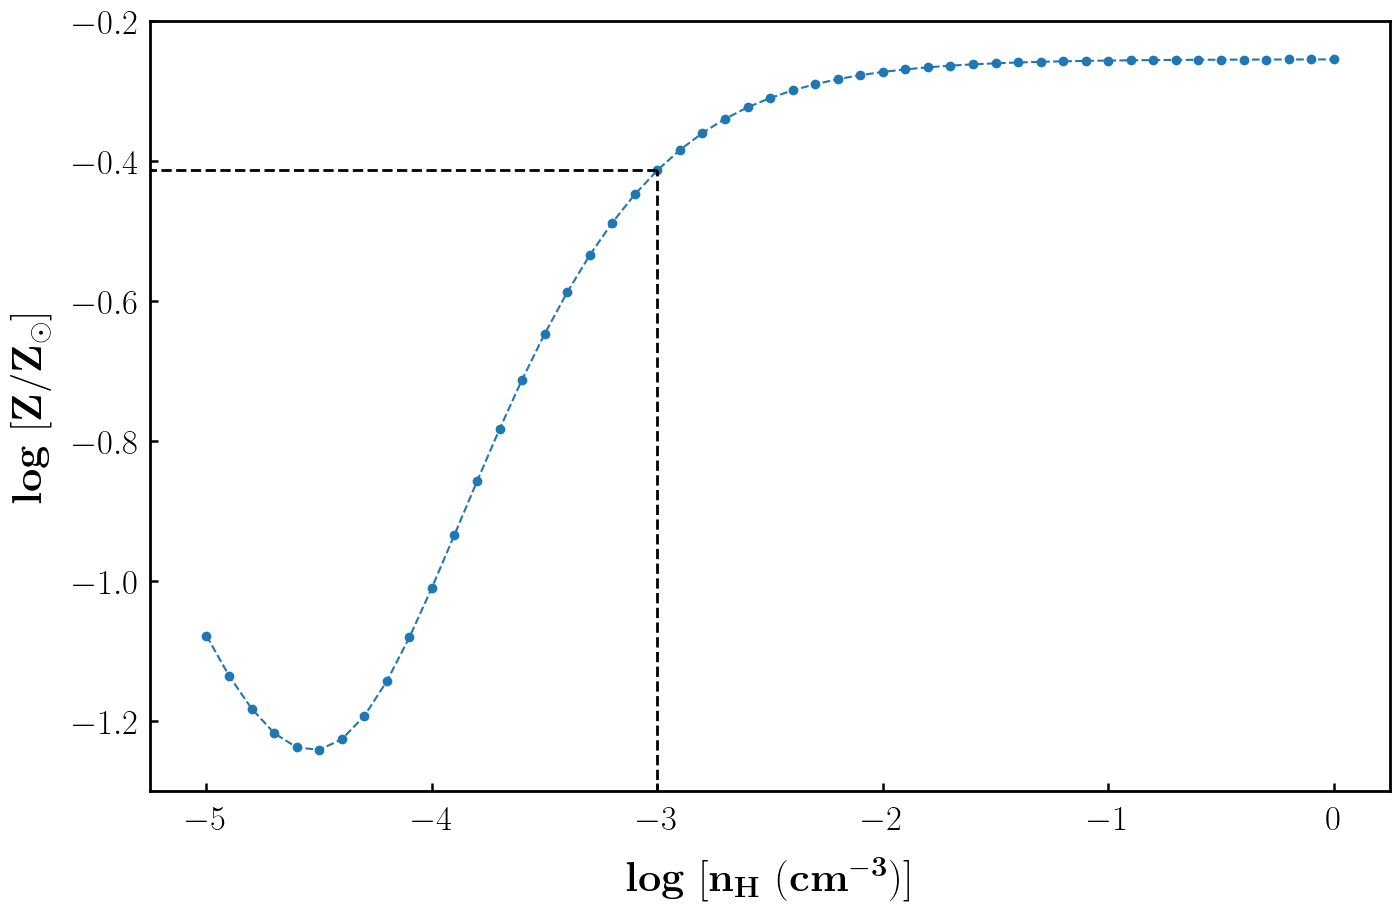
\includegraphics[width=\linewidth]{Figures/comp-II-CIE.png}
\caption{CIE solution for component II. The figure shows the metallicity found for various densities. At high densities no variation in metallicity is seen.}
\label{fig:comp_II_CIE}
\end{figure}

\subsection{Component III} \label{sec:compIII_modelling}

We consider only photionization modelling for this component, as small \emph{b} values indicate a low temperature for the component, as the contribution from collisional ionization will not be significant at low temperature.

\subsubsection{Photoionization modelling} \label{sec:compIII_PIE}

Along with \ion{H}{i}, we have 5 metal ion detections viz. \ion{C}{ii}, \ion{C}{iii}, \ion{Si}{ii}, \ion{Si}{iii} and \ion{O}{vi} in this component. We can estimate the density and metallicity for this component with the observed column densities of the detected metal ions by using CLOUDY models. As discussed in section \ref{sec:param-estimation} we use the $\chi^2$ minimisation technique described in \cite{acharya_khaire} to estimate the density ($n_H$) and metallicity (Z) of the absorber. We consider a dense grid of photoionization equilibrium (PIE) CLOUDY models with varying log $n_H$ and log Z. We vary the log $n_H \ ({cm}^{-3})$ from -5 to 0 in steps of 0.02 and log Z/${\text{Z}_\odot}$ from -3 to 2 in steps of 0.04 . The \ion{H}{i} column density for this component is log N(\ion{H}{i}) (${cm}^{-2}$) = 16.10 . So, we give the log [N(\ion{H}{i}) (${cm}^{-2}$)] = 16.10 as the stopping criteria for the CLOUDY calculations. The observed column densities and corresponding 1-$\sigma$ errors for the ions used in the process are listed in table \ref{tab:compIII}. The 1-$\sigma$ errors are the sum of errors given in table \ref{tab:col_den_error}, i.e we take in account the systematic uncertainty due to continuum fitting.
\\\\
We first try to model this absorber by assuming all the ions are arising from same gas phase, i.e. considering all the observed ions for $\chi^2$ minimization. We find that the solution can't match the modelled column densities with the observed column densities of the ions, except for \ion{O}{vi}, whose column density matches the best out of all the ions, as shown in figure \ref{fig:obs_predicted} (green filled circles). This predicts a temperature around $2.8\times 10^4$ K and a low density of log $n_H \ (\text{cm}^{-3})$ = -3.88 and total Hydrogen column density, $\text{log [N(H)} \ \text{cm}^{-2}]$ = 19.87, leading to a very large line of sight thickness of $\approx$ 180 kpc. 

\begin{table}
\centering
\begin{tabular}{ccc}
        \hline \hline
       \head{Ion} & \head{log[N (cm\textsuperscript{$\mathbf{-2}$})]} & \head{$\mathbf{\Delta}$ log[N (cm\textsuperscript{$\mathbf{-2}$})]} 
       \tabularnewline \hline \tabularnewline 
    \ion{O}{vi}      & 13.91 & 0.04  \tabularnewline \tabularnewline
    \ion{C}{ii}      & 14.21 & 0.39  \tabularnewline \tabularnewline
    \ion{C}{iii}     & 13.81 & 0.04  \tabularnewline \tabularnewline
    \ion{Si}{ii}     & 13.19 & 0.41  \tabularnewline \tabularnewline
    \ion{Si}{iii}    & 12.87 & 0.08  \tabularnewline
    \hline \hline \tabularnewline
 \end{tabular}
 \caption{Column densities and corresponding 1-$\sigma$ errors of the ions used in PIE modelling of the component III}
\label{tab:compIII}
\end{table}
%
%
\begin{figure}[!t]
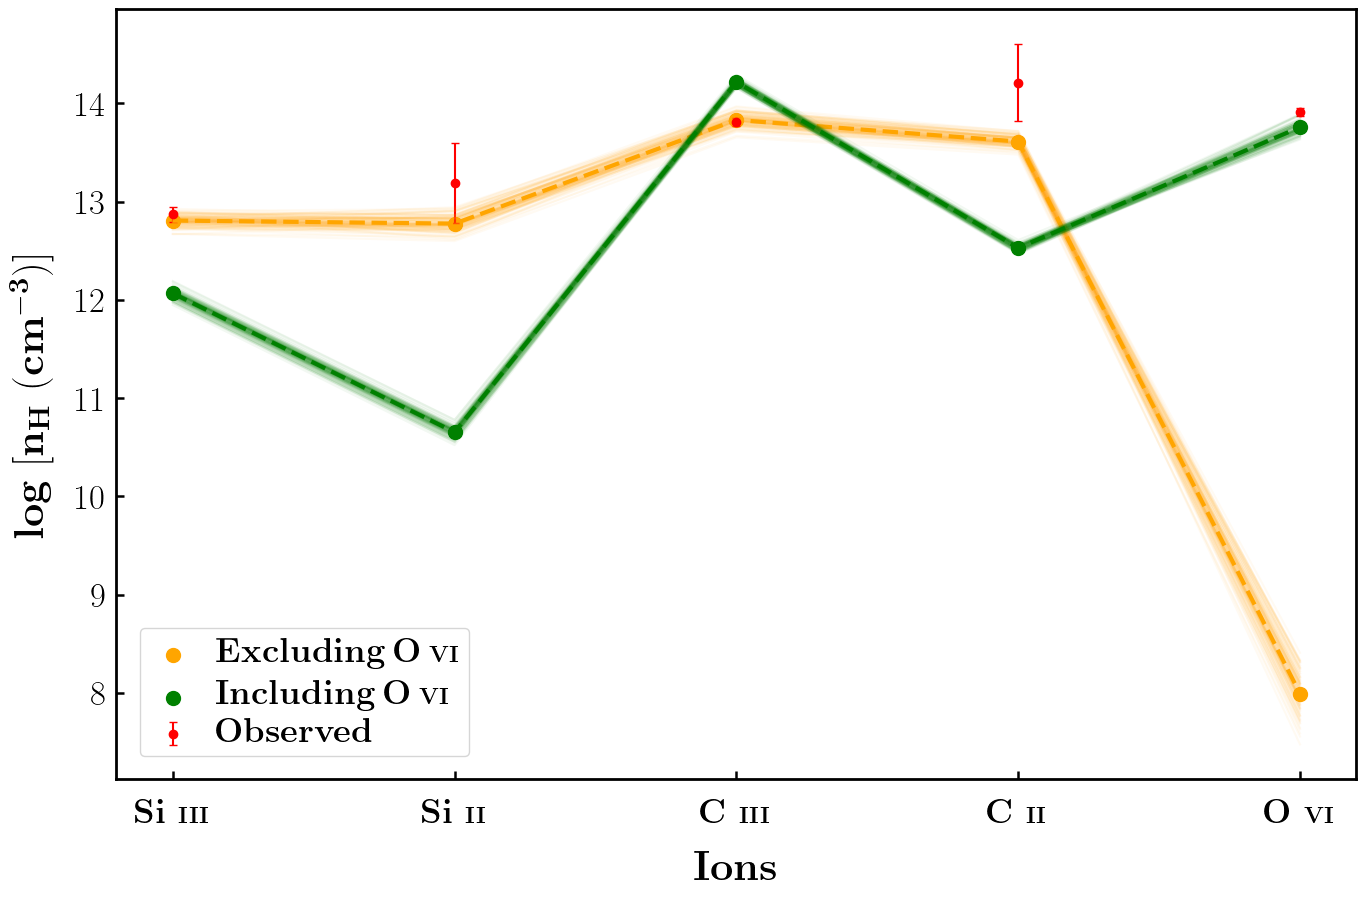
\includegraphics[width=\columnwidth]{Figures/Observed-and-predicted.png}
\caption{Modelled and observed column densities for the component III based on photoionization modelling. Red error bars shows the observed column densities and corresponding 1-$\sigma$ errors in column densities. The green and orange filled circles are the modelled column densities for the including \ion{O}{vi} and excluding \ion{O}{vi} case of PIE modelling. And the light green and light orange lines are modelled column densities with densities and metallicity sampled from normal distributions of log $n_H$ and log Z of including \ion{O}{vi} and excluding \ion{O}{vi} case respectively.}
\label{fig:obs_predicted}
\end{figure} 

As the above solution couldn't fit the observations well, we consider another case where all ions other than \ion{O}{vi} are arising from same gas phase. So, now we calculate the $\chi^2$ from column densities of other ions than \ion{O}{vi} and then minimise this $\chi^2$ to fit the model. This solution gives a good fit for the observed column densities of all the ions but now the \ion{O}{vi} is under-produced by orders of magnitude as seen in figure \ref{fig:obs_predicted} (orange filled circles) . This solution gives a temperature of about $1.0 \times 10^4$ K. This solution predicts a total Hydrogen column density, $\text{log [N(H)} \ \text{cm}^{-2}]$ = 17.92, smaller by nearly 2 orders than the previous case and a higher density, log $n_H \ (\text{cm}^{-3})$ = -2.24. This gives a line of sight thickness for the cloud to be around 50 pc.
As this case gives a better fit, we consider this to be the more correct description of the physical conditions in the absorber and draw our inferences based on this solution.

The log $n_H$, log Z and $\chi^2$ values for both the cases are given in table \ref{tab:compIII_PIE_sol}. And the physical properties of all the three components are listed in table \ref{tab:physical_param} based on the ionization modelling used.

\begin{table}[!htbp]
\centering
\begin{tabular}{cccc}
        \hline \hline
       \head{Case} & \head{log $\mathbf{n_H \ (\text{cm}^{-3})}$} & \head{log Z/$\mathbf{\text{Z}_{\odot}}$} & \head{$\mathbf{\chi^2}$}
       \tabularnewline \hline  
      All ions                  &  -3.88 $\pm$ 0.02    & -1.51 $\pm$ 0.03   &  275.67  \tabularnewline 
      Excluding \ion{O}{vi}     &  -2.24 $\pm$ 0.03    & -0.31 $\pm$ 0.06   &  4.27    \tabularnewline
     \hline \hline \tabularnewline
    \end{tabular}
\caption{Cloudy modelling solutions for absorber at z $\sim$ 0.34790. In case of all ions $\chi^2$ is calculated using the column densities of all the ions but for excluding \ion{O}{vi} ion case, $\chi^2$ is calculated by excluding \ion{O}{vi} column density so as to show that this fits other ions very well.}
\label{tab:compIII_PIE_sol}
\end{table}

\begin{landscape}
\thispagestyle{empty}
    
\begin{table}[!p]
\centering
\hspace*{-41mm}
\captionsetup{oneside,margin={0cm,15mm}}
\begin{tabular}{cccccccccc}
        \hline \hline \tabularnewline
        
      \head{Absorber}   & \head{Ions} & \head{log N({\text{H\,\small{\textsc{\uppercase{i}}}}})} & \head{Model}  & \head{log N(H)} & \head{log n\textsubscript{H}} & \head{log Z/$\mathbf{\text{Z}_{\odot}}$} & \head{Size} & \head{T} & \head{P/K} \\ \tabularnewline 
      \head{}   & \head{} & \head{$\mathbf{({cm}^{-2})}$} & \head{}  & \head{$\mathbf{({cm}^{-2})}$} & \head{$\mathbf{({cm}^{-3})}$} & \head{} & \head{(kpc)} & \head{(K)} & \head{$\mathbf{({cm}^{-3} \ K)}$} \\ \tabularnewline
      \hline \tabularnewline

z $\sim$ 0.34678                  &      \ion{H}{i}                          &  13.46                 &  -  &    -    &   -   &  -    &  -    &  $\leq \ 8.7 \times 10^4$  & -  \\ \tabularnewline

\multirow{2}{*}{z $\sim$ 0.34758} & \multirow{2}{*}{\ion{H}{i}, \ion{O}{vi}} & \multirow{2}{*}{14.13} & PIE &  18.45  & -4.51 & -0.31 & 29.47  & $2.5 \times 10^4$   & 0.77  \\
                                  &                                          &                        & Hybrid & $\lesssim$ 19.62  &  $\gtrsim$ -3   & $\gtrsim$ -0.4  & $\lesssim$ 13.35  & $1.9 \times 10^5$   & $\gtrsim $ 194.98  \\ \tabularnewline
                                  
\multirow{2}{*}{z $\sim$ 0.34790} & \multirow{2}{*}{\ion{H}{i}, \ion{O}{vi}, \ion{C}{ii}, \ion{C}{iii}, \ion{Si}{ii}, \ion{Si}{iii}} & \multirow{2}{*}{16.10} & PIE (All ions) &  19.87 & -3.88 & -1.51 & 180.75 & $2.8 \times 10^4$ & 3.68 \\
                   &                    &                    & PIE (Excluding \ion{O}{vi}) &  17.92 & -2.24 & -0.31 & 0.05 & $1.0 \times 10^4$ & 59.02 \\ 

        \tabularnewline \hline \hline \tabularnewline
    \end{tabular}
\caption{Physical properties of the absorbers based on Voigt profile measurement and CLOUDY ionisation modelling. The PIE solution for absorber at z $\sim$ 0.34758 is based on the excluding \ion{O}{vi} case PIE solution of the absorber at z $\sim$ 0.34790.}
\label{tab:physical_param}
\end{table}

\end{landscape}



\section{Origin of {\text{O\,\small{\textsc{\uppercase{vi}}}}} in the Absorber}


\subsection{Component II} \label{sec:temp_calc_b}

The large \emph{b} value indicates a large value of the temperature. As we the \ion{O}{vi} absorption is coincident with the BLA we can directly estimate this temperature using their \emph{b} values. The \emph{b} values which we get from Voigt profile have both thermal and non thermal contributions. 
\begin{equation} \label{eq:b_HI}
\emph{b}(\ion{H}{i})=\sqrt{{{\emph{b}^2}_{\text{thermal}}(\ion{H}{i})}+{{\emph{b}^2}_{\text{non-thermal}}}}
\end{equation}
\begin{equation}
\emph{b}(\ion{O}{vi})=\sqrt{{{\emph{b}^2}_{\text{thermal}}(\ion{O}{vi})}+{{\emph{b}^2}_{\text{non-thermal}}}}
\end{equation}
\begin{equation} \label{eq:b_thermal}
\emph{b}_{\text{thermal}}=\sqrt{\frac{2kT}{m}}
\end{equation}
Where, $k, \ T \text{and} \ m$ are Boltzmann constant, temperature and atomic mass of the species respectively.
\\\\
From equation \ref{eq:b_thermal} we have,
\begin{equation}
{\emph{b}}_{\text{thermal}}(\ion{H}{i})=4\ {\emph{b}}_{\text{thermal}}(\ion{O}{vi})
\end{equation}
Solving above equations for T gives, $T={10}^{{5.29}_{-0.08}^{+0.07}}$ K, which lies in the temperature range of WHIM. This temperature results in ${\emph{b}}_{\text{thermal}}$(\ion{H}{i}) $\sim 57 \ \text{km} \  \text{s}^{-1}$ and ${\emph{b}}_{\text{thermal}}$(\ion{O}{vi}) $\sim 14 \ \text{km} \  \text{s}^{-1}$. High temperature contributes to around 91 \% of the broadening of the \ion{H}{i} line whereas the \ion{O}{vi} line broadening is dominated by non-thermal components. An inherent assumption in this calculation is that the both lines have same contributions from non-thermal components. 

The ionization fraction of \ion{O}{vi} in collisional ionization equilibrium peaks around $10^{5.7}$ K. We are getting a nearby temperature of ${10}^{5.29}$ K, so the \ion{O}{vi} could be tracing a collisionally ionised gas phase. 

\subsection{Component III}

As discussed in section \ref{sec:compIII_PIE}, we consider two cases of photoionization models, one solution is able to explain \ion{O}{vi} column density but can't model column densities of other ions. Another solution models the column densities of other ions but fails to explain the \ion{O}{vi} column density. We discard the first case on grounds of poor fit and large line of sight length. And accept the second case to be more accurate description of the absorbing cloud conditions. We argue that as the other ions excluding \ion{O}{vi} can be explained by photoionisation models, they must be arising from a cool photoionised gas phase. But the question still remains that from where the \ion{O}{vi} absorption is coming from ?  

There have been similar instances in literature where the \ion{O}{vi} can't be explained from photoionised phase and could possibly be tracing a warm phase \citep[see e.g.][]{Pradeep-2020,Anshul-2021}. So,
we assert that \ion{O}{vi} absorption may be arising from a different hidden phase in the absorber and possibly tracing a collisionally ionised phase. However, to infer about this 'hidden' phase we need details on the associated Lyman $\alpha$ component. Since the Lyman $\alpha$ feature in absorber system is almost saturated with 3 components, we can't get any insights on the contributions from the hidden $\text{4}^{\text{th}}$ component if there is any.

\section{Galaxy environment of the absorber}

Galaxies, galaxy groups or clusters can have large gaseous halos surrounding them, called the circumgalactic medium (CGM) extending upto kpc scales. Our absorber system could be tracing one such halo. So we lookout for the galaxies around the absorber to check if this is the case. We search galaxies with velocity separations within 1000 km $\text{s}^{-1}$ from the absorber and within 15$\arcmin$ on the plane of sky from the quasar line of sight, which spans around 4.4 Mpc at the absorber redshift \footnote{Assuming a flat $\Lambda$CDM cosmology with $\text{H}=69.6 \ \text{km} \ \text{s}^{-1} \ \text{Mpc}^{-1}$}. No spectroscopically identified galaxies were found in the SDSS DR17 \citep{SDSS_DR17} footprints with above constraints.  SDSS' 90 per cent spectroscopic completeness limit of r < 17.8 \citep{strauss_SDSS} gives luminosity limit of L $\gtrsim$ 2.77 $\text{L}^{*}$ at z $\sim$ 0.347 assuming luminosity functions calculated by \citet{ilbert_GLF}. This implies that the SDSS spectroscopic survey has only sampled the bright galaxies only. So there could be sub-$\text{L}^{*}$ galaxies present around the absorber system

Our line of sight was also observed under the VIMOS survey \citep{vimos_data} (PI - Thomas Shanks, Program Id : 097.A-0535(D)). The VIMOS field of view in imaging mode comprises of 4 quadrants. The quasar PG0003+158 was centered in the $\text{3}^\text{rd}$ quadrant out of this 4 quadrants. The field was observed in B (383-478 nm) and R (579-713) filters.

\begin{table}[!t]
\centering
    \begin{tabular}{cccccccc}
        \hline \hline
       \head{R.A.} & \head{Dec.} & \head{z} & \head{$\mathbf{\Delta v}$} & \head{$\mathbf{\eta}$} & \head{$\mathbf{\rho}$}  & \head{r} & \head{L} \\ 
        &  &  & \head{$\mathbf{(\text{km \ s}^{-1})}$} & \head{(arcmin)} & \head{(Mpc)}  &  & \head{($\mathbf{L^*}$)}
       \tabularnewline \hline  \tabularnewline
        1.43341  &  15.97131  &  0.3351  &  -2564  &  12.1  &  3.6  &  20.387   &  0.24   \\
        1.52570  &  15.98456  &  0.3466  &  -200  &  10.9  &  3.2  &  21.719   &  0.07  \\
        1.48286  &  16.14235  &  0.3517  &  838  &  1.5  &  0.4   &  21.533   &  0.09  \\
        1.43069  &  16.16771  &  0.3582  &  2153  &  3.8  &  1.1  &  19.342   &  0.72  \\
        1.44071  &  16.16933  &  0.3593  &  2374  &  3.3  &  1.0  &  19.745   &  0.50  \\
       \tabularnewline \hline \hline 
    \end{tabular}
\caption{Galaxies in the neighbourhood of the absorber system identified in VIMOS survey. Velocity is taken to be zero at z = 0.347586}
\label{tab:galaxies}
\end{table}

5 galaxies were identified within the field. We looked for these galaxies in the SDSS photometric survey and found all of the 5 galaxies providing us with the photometric data. The details of the galaxies are given in table \ref{tab:galaxies}. The table gives the position, redshift, velocity separation, separation on the plane of sky ($\eta$) , projected distance on the plane of sky ($\rho$) and the SDSS r-band magnitude and luminosity of the galaxies. Two of the galaxies were within 1000 km $\text{s}^{-1}$ and 15$\arcmin$ from the quasar line of sight. Figure \ref{fig:galaxy} shows the galaxies around the absorber system color coded with the absolute velocity separation from the absorber system (z=0.347586). The cross mark in the center is the line of sight of PG 0003+158. The blue and orange dashed curves show the projected distance at the absorber redshift (z=0.347586) of 500 kpc and 1 Mpc respectively. There is one galaxy within a projected separation of 500 kpc but it separated by around 838 km $\text{s}^{-1}$ from the absorber. We find one galaxy at 200 km $\text{s}^{-1}$ from the absorber but it is at a projected distance of around 3.2 Mpc from the line of sight. 

\begin{figure}[!t]
% \vspace{-40mm}
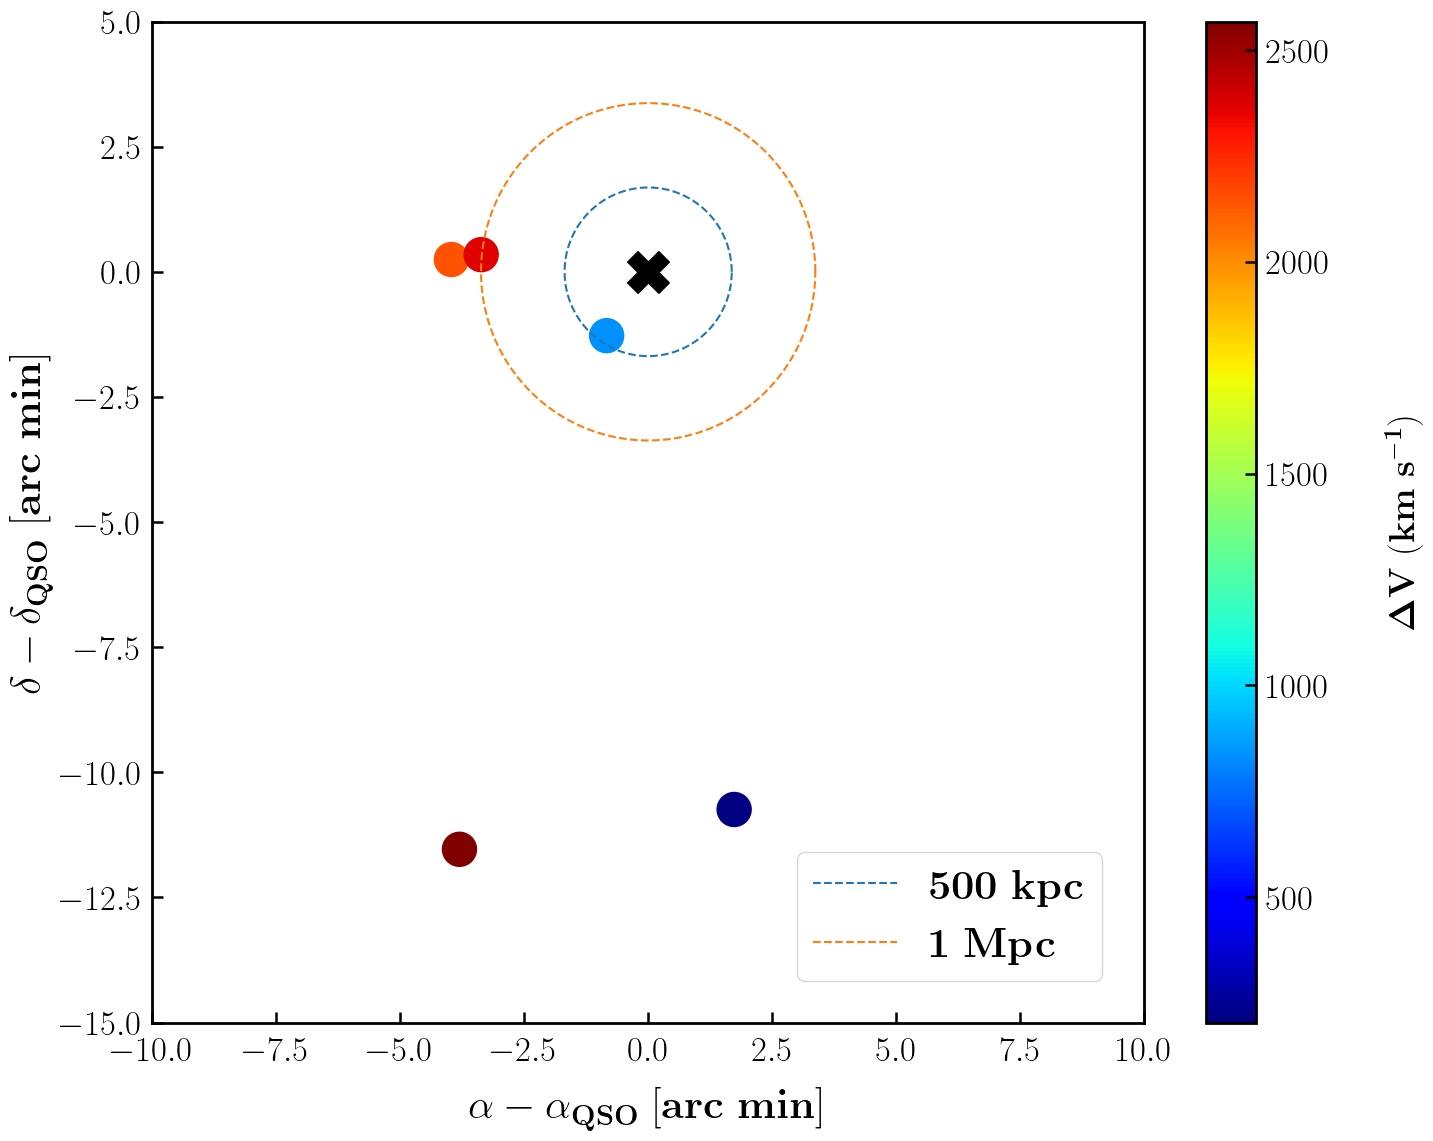
\includegraphics[width=\columnwidth]{Figures/galaxy_environment.png}
\caption{Galaxies around the absorber color-coded with their velocity separation from the absorber.}
\label{fig:galaxy}
\end{figure}

\citet{Prochaska-2011} gives the following scaling relation between luminosity and virial radius of a galaxy but warns that this is based on crude estimates and should serve as a mere guideline:

$$r_{vir}=r^{*}_{vir}\left(\frac{L}{L^{*}}\right)^{\beta}$$

with $r^{*}_{vir}=250$ kpc and $\beta=0.2$. For the galaxy at projected distance of 0.4 Mpc which is the closest in projected distance, $r_{vir}$ comes out to be 155 kpc which is 2.6 times less than the projected distance. So the absorber is quite far from the CGM of this galaxy. The virial radii of other galaxies are also not large enough.

We see that the absorber lies in a galaxy under-dense region, so the absorber could be tracing a large scale filamentary structure in the cosmic web or CGM of a faint galaxy with a luminosity less than 0.07 L$^*$ which is not sampled in the current observations.



